\textbf{Download the program \textsc{wave2D\_leap\_frog.m}. This code solves the wave equation,
\begin{align*}
u_{tt}=u_{xx}+u_{yy},~~~~(x,y)\in [-1,1]\times [-1,1],~~t>0,
\end{align*}
with homogeneous Dirichlet boundary conditions and initial conditions
\begin{align*}
u(0,x,y) = exp(-40((x−0.2)^2+y^2)),~~ u_t(0, x, y) = 0.
\end{align*}
Modify this code to solve the same problem but with homogeneous Neumann boundary instead of Dirichlet. Plot your solution at time $t= 10$. How accurate is your solution? (number of digits)
}
\newline

To impose homogeneous Neumann boundary conditions we can simply ignore some rows and colums on our matrix multiplications. Taking $u_{yy}$:
\begin{align*}
u_{yy} = DDu = Du_y,
\end{align*}
where $D$ is the Chebyshev differentiation matrix. We know that $u_y$ has zero components in the first and last rows. This allows us to ignore the first and last rows of $D$ when taking the first multiplication. In addition, we can also ignore the first and last column of the second multiplication. Hence, we can simply impose Neumann boundary conditions by making,
\begin{align*}
u_{yy} = D(:,2:N)D(2:N,:)u,
\end{align*}
following \textsc{Matlab} notation. Analogous discussion can be made about $u_{xx}$, obtaining
\begin{align*}
u_{yy} = uD(2:N,:)'D(:,2:N)',
\end{align*}
where the $D'$ represents the transpose of $D$. The solution at $t=10$ is shown in the next figure.

\begin{figure}[H]
\centering
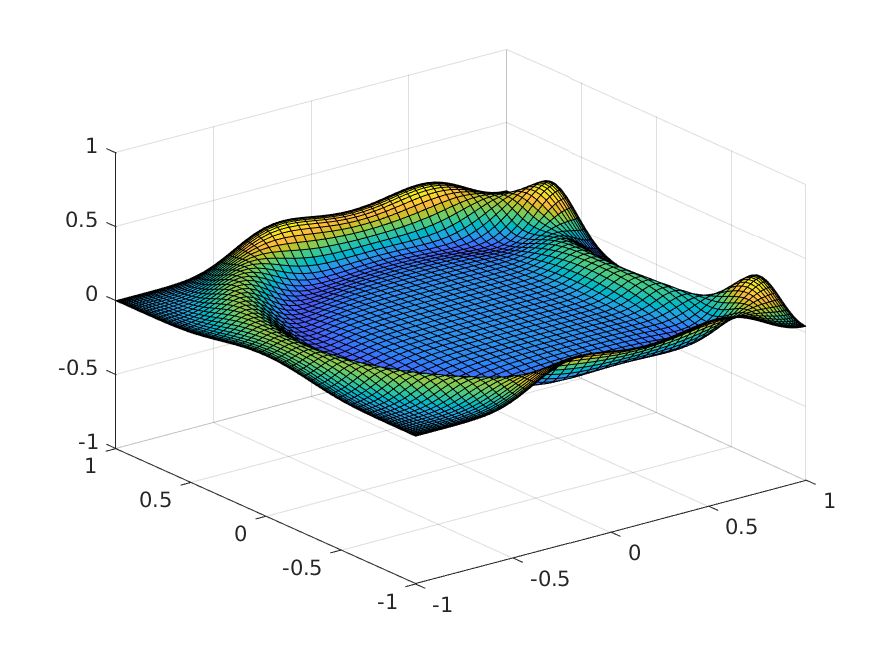
\includegraphics[scale=0.75]{P4.png}\caption{WRITE CAPTION.}
\end{figure}

\subsection*{Matlab code for this problem}
\begin{verbatim}
%% Homework 4, Problem 4 -  Francisco Castillo
clear all; close all; clc
labelfontsize = 14;
%% 2D wave equation Chebyshev+Leap-frog, ZERO Neumann BC'S
N = 64;
[D,x] = cheb(N);
% x = x(2:end-1);
% D2 = D^2;
% D2 = D2(2:end-1,2:end-1);
 
% 2D grid
[X,Y] = meshgrid(x);
 
% Initial condition
u0 = exp(-40*((X-0.2).^2+Y.^2));
u = u0;
 
h = 1-x(2);
dt = h/2;
t = 0;
tf = 10;
count=0;

while t<tf
    if t+dt>tf
        dt = tf-t;
    else
        dt = h/2;
    end
    uyy = D(:,2:N)*D(2:N,:)*u;
    uxx = u*D(2:N,:)'*D(:,2:N)';
    u2 = 2*u- u0 + dt^2*(uxx+uyy);
    u0 = u;
    u = u2;
    
    if count == 10 
        surf(X,Y,u)
        zlim([-1 1])
        drawnow
        shg
        count = 0;
    end
        
    count = count+1;
    t = t+dt;
    
    if t == tf
        surf(X,Y,u)
        zlim([-1 1])
        drawnow
        shg
        xlabel('$x$','interpreter','latex','fontsize',labelfontsize)
        ylabel('$y$','interpreter','latex','fontsize',labelfontsize)
        zlabel('$u(x,y)$','interpreter','latex','fontsize',labelfontsize)
        set(get(gca,'ZLabel'),'Rotation',0)
        saveas(gcf,'Latex/FIGURES/P4','png')
    end
end
\end{verbatim}